% !TeX spellcheck = en_US
\documentclass[a4paper,twoside]{article}

\usepackage{epsfig}
\usepackage{subcaption}
\usepackage{calc}
\usepackage{amssymb}
\usepackage{amstext}
\usepackage{amsmath}
\usepackage{amsthm}
\usepackage{multicol}
\usepackage{pslatex}
\usepackage{apalike}
\usepackage{SCITEPRESS}

% user packages
\usepackage{url}

\usepackage{graphicx}
\usepackage{colortbl}
\usepackage{xcolor}

\usepackage{listings}
% setup for C and C++
\lstset{
	numbers=left,                   % where to put the line-numbers
	stepnumber=1,                   % the step between two line-numbers.        
	numbersep=3pt,                  % how far the line-numbers are from the code
	numberstyle=\tiny,				% size of the line-numbers
	backgroundcolor=\color{white},  % choose the background color. You must add \usepackage{color}
	showspaces=false,               % show spaces adding particular underscores
	showstringspaces=false,         % underline spaces within strings
	showtabs=false,                 % show tabs within strings adding particular underscores
	tabsize=2,                      % sets default tabsize to 2 spaces
	captionpos=b,                   % sets the caption-position to bottom
	breaklines=true,                % sets automatic line breaking
	breakatwhitespace=true,         % sets if automatic breaks should only happen at whitespace
	title=\lstname,                 % show the filename of files included with \lstinputlisting;
	basicstyle=\ttfamily,			% style of the whole listing
	showstringspaces=false,			% do not show spaces in strings
	keywordstyle=\color{blue}\ttfamily,
	stringstyle=\color{red}\ttfamily,
	commentstyle=\color{teal}\ttfamily\textbf,
}


\begin{document}
	
\title{DDoS Mechanisms Simulations and Performance Comparison}

\author{\authorname{Bruno Neves, Filipe Mourão, Lucas Jorge, Rahyan Azin, Juliana Bezzera and Vitor Curtis}
	\affiliation{Department of Computer Science Department, ITA, São José dos Campos, Brazil}
	\email{\{neves.brunobr, filipemleite94, lucas1jorge, rahyan.azin\}@gmail.com, \{juliana, curtis\}@ita.br}
}

\keywords{DDoS, botnet, election, network topology.}

\abstract{The concern about cyber security has attracted attention by organizations and public services over the last few years due to the contemporary importance of confidentiality, integrity, and availability of services and sensitive data. In contrast, many recent episodes of cyber attacks causing strong impact were performed using extremely simple techniques and taking advantage of the hidden weaknesses of current systems. This article has the main purpose to motivate the academy to mitigate such unexpected potential cyber attacks from the attacker's perspective, exposing the latent weakness of current systems, since the majority of such papers focus only on the defense perspective. We analyze the potential impact of Denial of Service (DoS), a very popular cyber attack to affect the availability of a victim server, through different mechanisms and topologies. Specifically, we simulate and analyze the impact of Distributed DoS (DDoS), a more powerful kind of DDoS, when using the List and Binary Tree topologies with Continuous or Pulsating stream of requests, and finally, we introduce a simple new technique to improve the DDoS against mitigation.
% Vitor: O foco original do artigo é sobre uma comparação de performance entre duas topologias de botnet para ataques DDoS.
% Vitor: Justificar a escolha das duas topologias, e comentar os dois tipos de pulsos.
% The effect of the delay in network propagation while coordinating a wave attack in the botnet is made evident when comparing the mechanisms, and the package loss in the attacked server could be observed in the simulations.
% Vitor: achado da pesquisa que deve ser explorado nos resultdos. No abstract é muito estranho, pois falta todo o contexto da pesquisa.
%This type of experience is not easy to find in academic studies, since they usually focus on defense and mitigation of attacks, and thus it offers a valuable didactic learning.
% Vitor: acho que a motivação do trabalho pode ser alterada para a relevância do impacto de DoS.
}

\onecolumn \maketitle \normalsize \setcounter{footnote}{0} \vfill

\section{\uppercase{Introduction}}

\noindent Over the last decade, we have seen technologies as streaming, deep learning, IoT, blockchain and big data disrupting traditional business and enabling a prolific market of network-based systems where data are the principal value. In this context, secure and reliable systems are very important to not tarnish the image of a company and crucial in critical systems and public services.

A good example of potential damage a network cyber attack could lead was recently revealed by \cite{McCallie:2011}. They expose the fragility of the Automatic Dependent Surveillance-Broadcast (ADS-B) system of the global air traffic control. Using about \$1,000 worth of radio equipment, a hacker could simply flood the air traffic control system with as many fake airplanes as it wants.

In 2016, Mirai botnet attacked the Internet Service Provider (ISP) for sites such as Twitter, Amazon, PayPal, Spotify, Netflix, and others, making them unreachable for several hours. In such attacks, a worm propagates through networks and systems taking control of poorly protected IoT and embedded devices such as IP cameras, thermostats, Wi-Fi enabled clocks and washing machines \cite{Kolias:2017}. At its peak, Mirai infected over 600,000 vulnerable devices and was able to attack the OVH services with a volume of network traffic around 1Tbps \cite{Antonakakis:2017}.

These episodes expose considerable negligence by companies in the past years regarding security, which now reflects as latent threats to computer systems. Forecastings estimate that IoT and small devices will represent more than 75\% of the global Internet reaching 10 billion in 2020 and representing a true potential threat specially because of new connected solutions with poor security pop up every day by small business and startups, \cite{Rose:2015}, \cite{Columbus:2018}.

With this scenario, we propose that the academy encourage more research papers from the attacker's perspective rather than the defense to force the exposure of current hidden weaknesses of computer systems as a measure of prevention from real potential attacks to organization and states.

According to \cite{Schatz:2017}, the current terminology to discuss security aspects of digital devices and information is cyber security and it is basically defined as the actions and technologies followed by organizations and states to protect confidentiality, integrity, and availability of data and assets used in cyberspace.

Among the cyber threats, the Denial-of-Service (DoS) is a very easy and common kind of cyber attack that violates the availability of systems. Besides it looks harmless at first, as cited by the examples above, it can cause severe damages to organizations and public services. Furthermore, due to the contemporary importance of confidentiality and value of data, cyber attacks can cause an important devaluation of brands by inducing distrust about the integrity and confidentiality of personal data or services, becoming even a tool to commit financial crimes by influencing the stock markets.

In this article, we motivate the attacker's philosophy of cybersecurity by analyzing the performance of some Distributed DoS (DDoS), a non-trivial kind of DoS, as a way to analyze the potential damage a real scenario powered by the growth of IoT devices could cause.

First, we present some basic concepts of DoS and DDoS in section \ref{sec:basic}, followed by a common taxonomy of the main methods of DDoS based on some behavior mechanisms. Section \ref{sec:simulation} describes how to simulate the main methods of DDoS introduced in the previous section and the limitations of these simulations. Section \ref{sec:evaluation} discusses the results of the simulations and the potential of each mechanism. In section \ref{sec:protection}, we propose a new technique difficulting DDoS mitigation by protecting the attacking network and, finally, \ref{sec:conclusion} cites the main conclusions of this work.

\section{\uppercase{Basic concepts of DoS and taxonomy of DDoS}} \label{sec:basic}

DoS is a cyber-attack in which the perpetrator seeks to make a machine or network resource unavailable to its intended users by temporarily or indefinitely disrupting services of a host connected to the Internet \cite{Soltanian:2016}, and it can be achieved by different methods. A simple example of DoS with limited side effect is deliberately entering a wrong password enough consecutive times to cause the victims account to be locked.

Usually, the most common method of attack occurs when the hacker floods a network server or resource with superfluous or incorrect requests in an attempt to decrease its availability to attend legitimate requests and blocking all users at once. One example of such attack is known as SYN flood, where one sends a request to connect but never completes the connection through a three-way handshake. The incomplete handshake leaves the connected port in an occupied status and unavailable for further requests.

Many of these DoS attacks are easy to identify and block by only checking the source of the requests. Because of this, hackers usually use DDoS, which implements distributed computing to coordenate multiple attackers from different sources to send malicious traffic to a targeted server.

\begin{figure}[h]
	\centering
	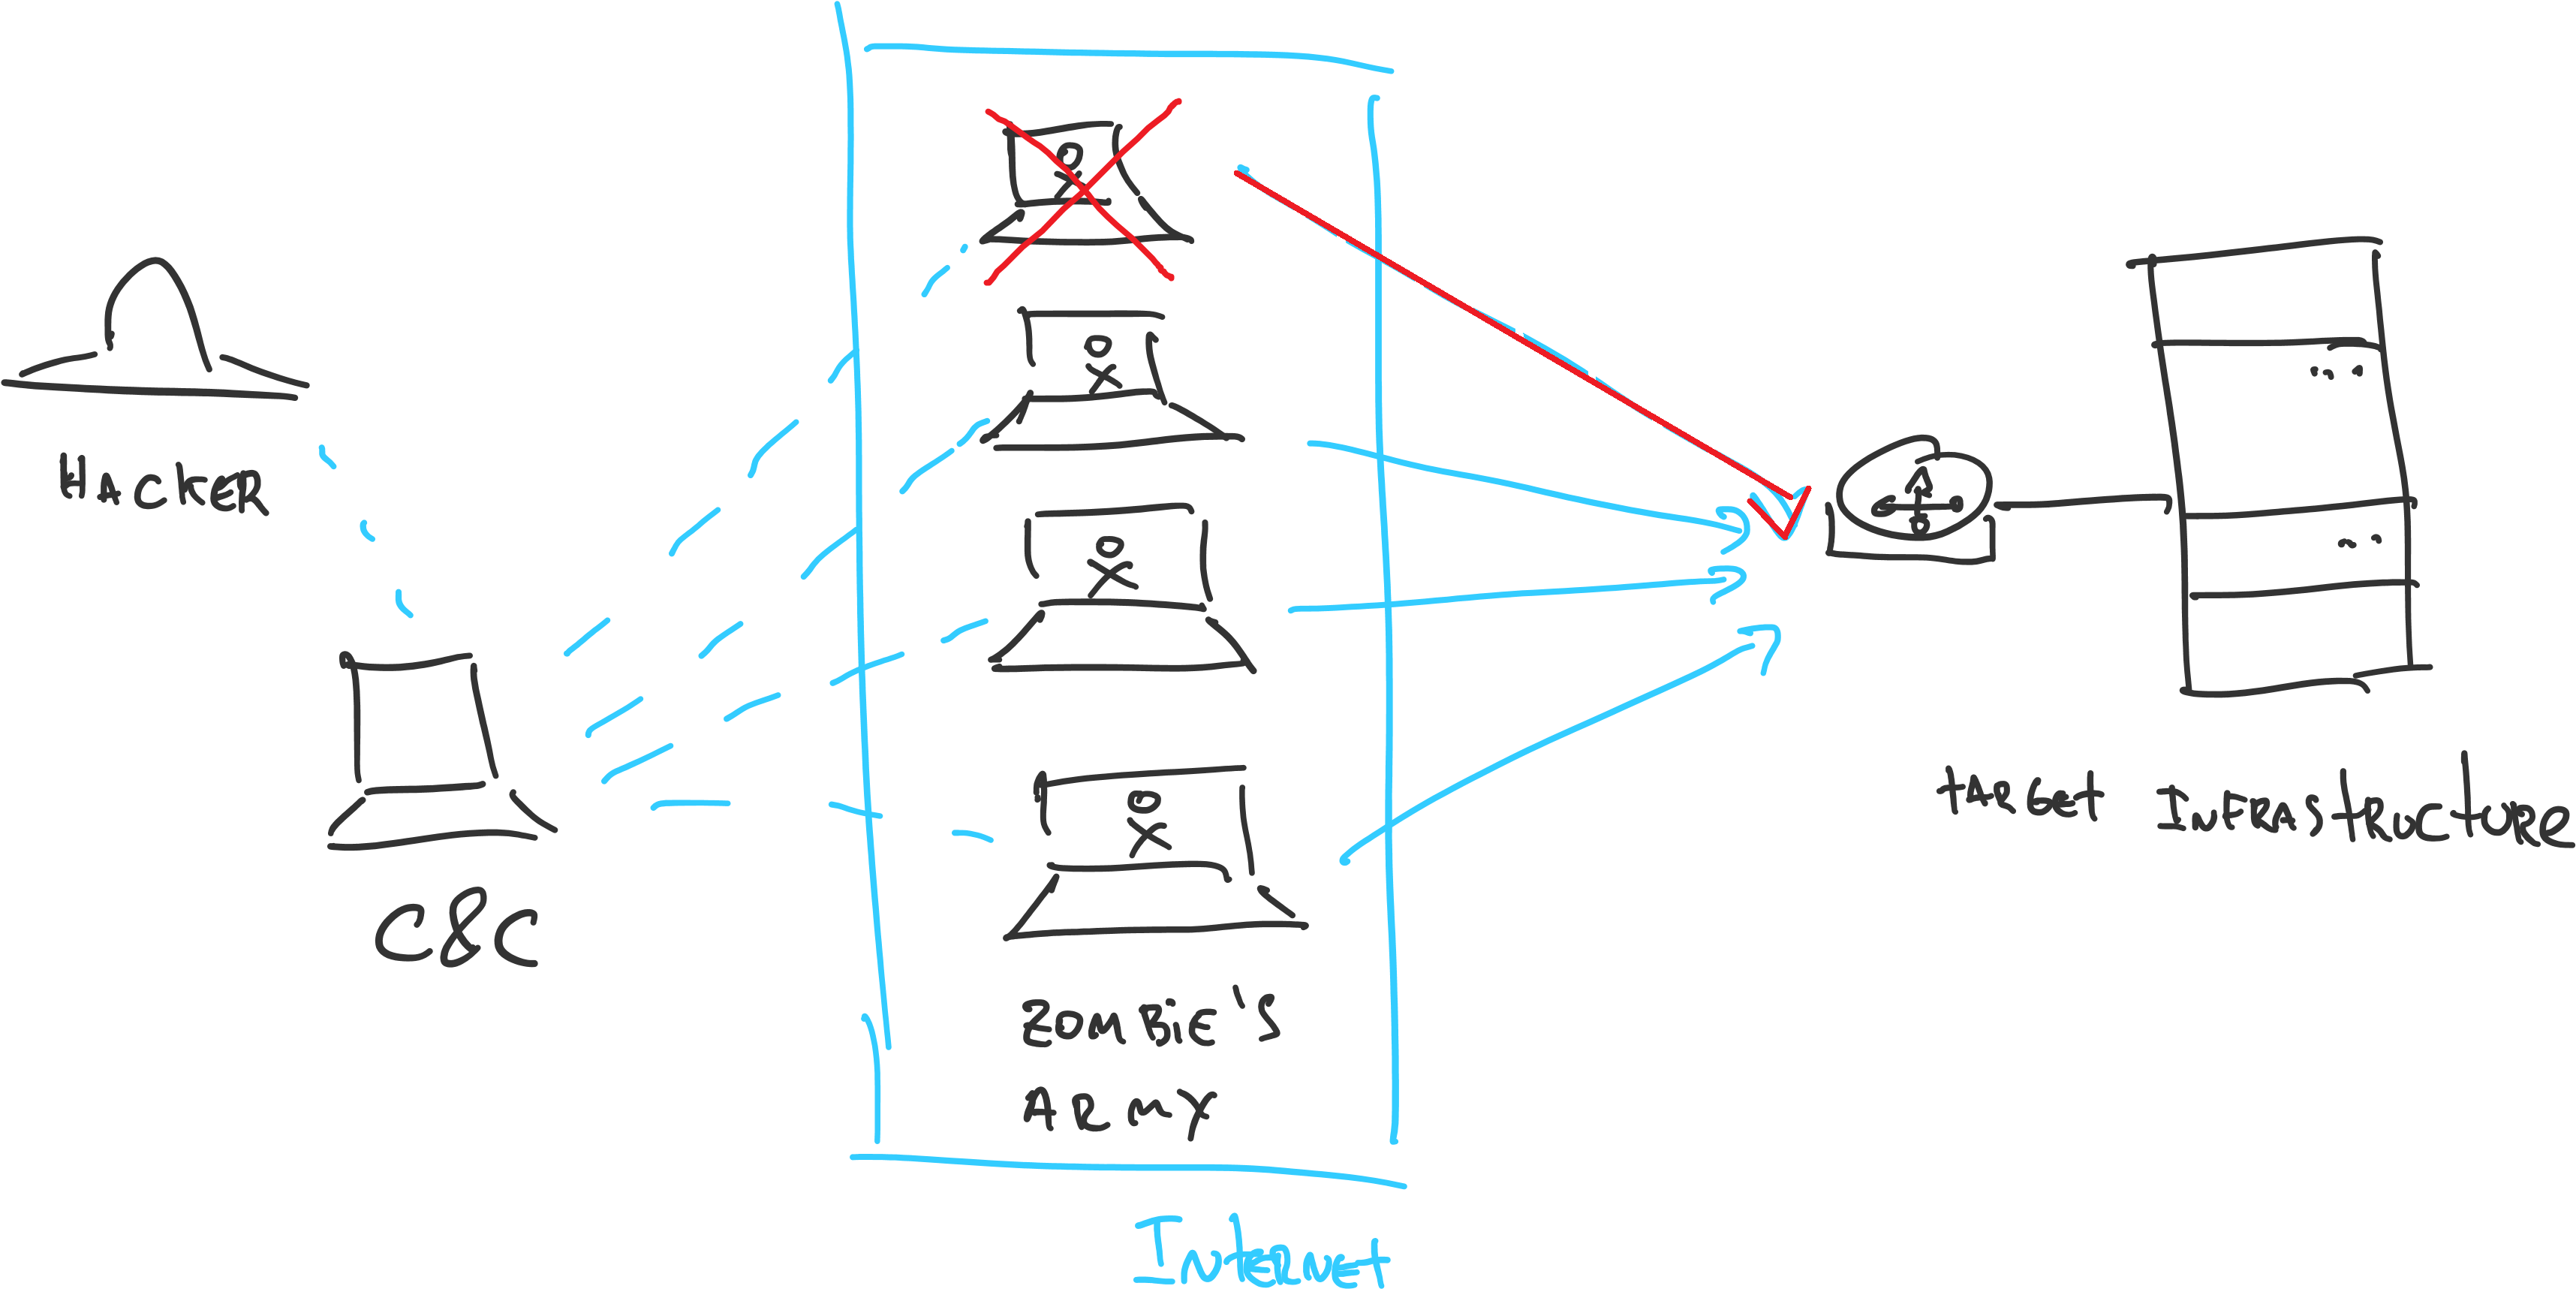
\includegraphics[width=.9\linewidth]{img/DDoS-arch}
	\caption{Arquitecture example of a DDoS botnet with one zombie, in red, blocked by the target firewall.}
	\label{fig:DDoS-arch}
\end{figure}

A DDoS starts with the hacker first spreading malicious softwares called malware with the intention to infect an army of Internet-connected devices, named zombie computers, with backdoors running in background and waiting for commands from a Command and Control (C\&C) server, as shown in Figure \ref{fig:DDoS-arch}, configuring a network of zombies called botnet.

After many devices invected, the hacker initiates a DDoS through the C\&C, which is responsible to spread the attack command over the botnet, and each zombie perfoms the attack by requesting some service over the network to the target infrastructure. It becomes the defence much more difficult since blocking one IP, see Figure \ref{fig:DDoS-arch}, has almost no effect because of the massive amount of attacking points spread over the Internet.

DDoS is also much more powerfull than a simple DoS because it multiplies the capacity of sending fake request to the target, the massive amount of available resources enables requests with signatures very close to genuine requests, and it can be implemented with no central point of C\&C, making the interruption of an attack much more difficult.

In the literature, there are some taxonomies trying to capture all the methods involving DDoS. \cite{Mirkovic:2004} and \cite{Bhardwaj:2016} classify DDoS by ... \emph{descrever os tipos principais de classificação: degree of automation, exploration of vulnerability, attack rate dynamic (ARD) and attack impact, além de comentá-las brevemente. De preferência, adicionar uma imagem das classificações dos autores}.

We focus the analysis of our simulations in DDoS with ... \emph{comentar as classes escolhidas para serem analisadas no trabalho, com exceção das classes DA e ARD que terão suas subseções específicas por serem as mais importantes. Nota: Algumas classes não tem muito o que falar. Apenas citar e justificar simplesmente}.

Following, the subsections \ref{sec:da} and \ref{sec:ard} respectively describe in more details the mechanisms of DA and ATD analysed in our simulation.

\subsection{\uppercase{Degree of automation}} \label{sec:da}

The semi-automatic degree of automation ... \emph{justificar o modo semi-automático implementado, suas relações com a topologia e apresentar o problema de se esconder a estrutura da rede de zombies para evitar contra-ataque: os zumbies apenas se comunicam com o C\&C durante a fase de ataque. De preferência, adicionar uma diagrama para explicação}.

\emph{Ajustar a questão da topologia, comentado com \% abaixo, para continuar explicação do nível de automatização pretendido no trabalho: foco em ser o mais automático possível, porém com início de ataque manualmente controlado pelo hacker}.

% ajustar texto abaixo para fluir como o acima
%Botnets can be formed in different network structures (topologies), for which the most common are:
%\begin{itemize}
%	\item Star topology: There is a central Command and Control (C\&C) server, with the bots organized around it;
%	\item Hierarchical topology: Bots organized in layers of C\&C servers;
%	\item Random topology: peer-to-peer communication	between bots (P2P).
%\end{itemize}
%An unwanted weakness in the centralized topologies is the vulnerability of having the central C\&C taken down. An advantage to be explored from the Random topology (P2P) is the resiliency, the capability of reorganizing some bots in case of an eventual failure of a near server.
%In case of failure in the tree topology, an election algorithm was designed to replace the missing node with one of its children, with the intention of maintaining the functionality and lower the vulnerability of the network architecture. In case of failure in the list topology, it’s enough to assume that the failing node is removed and it’s left and right neighbors establish a connection.

In order to preserve the manual control of the attack, in section \ref{sec:protection}, we propose a new method of automation which controls the botnet with resilience against mitigation, where zombies have only partial information about the topology.

\subsection{\uppercase{Attack rate dynamics}} \label{sec:ard}

A DDoS can also follow different dynamics depending on the duration, form, and distribution of the traffic in the stream of superfluos requests, where the more similar its signature is to a genuine request, the more difficult it is to detect the DDoS. A taxonomy with two main classes of ARD patterns are described in \cite{Liu:2012}.

% explicar em maiores detalhes cada uma das grandes classes, bem como suas consequências e justificar quais serão utilizadas nas simulações.

%First, Flood DoS (FDoS): Keep sending a high rate traffic to the victim. The traffic of requests can follow different dynamics, commonly establishing constant, increasing or fluctuating rate stream:

%Figure 1 em vetor

% Second, Low Rate DoS (LDos): send short bursts of traffic, with a duration predetermined maliciously and a frequency related to the retransmission timeout (RTO) of the packages in the network, so that the victim stays in a superfluous retransmission trap. Common dynamics of LDoS are the square-wave, two rate square-wave and sine waveforms:

%Figure 2 em vetor

%In this work, the two common mechanisms of DoS will be implemented: Continuous stream DDoS and Pulse wave DDoS. Then, each mechanism will be used in two topologies: tree and list. Finally, we’ll compare their performances in disrupting the services and causing package loss in the targeted server.

\section{\uppercase{Simulations of DDoS}} \label{sec:simulation}

\emph{Reescrever a seção explicando as simulações esolhidas no trabalho e como foram desenhadas, porém sem apresentar nenhuma informação sobre sua implementação. A implementação e manual de uso das ferramentas desenvolvidas não são relevantes e não devem estar contidas no artigo. Caso o leitor queira saber sobre a implementação e uso, irá verificar as informações no Git. Adicionar uma frase indicando o endereço onde o leitor poderá encontrar as informações de uso e todos os resultados das simulações}

\emph{Na apresentação, foque nos conceitos principais das tomadas de decisão e tente generalizar o máximo possível as simulações para outros cenários. Novamente, não esqueça de justificar tudo o que for dito. Se alguma informação for adicionada na justificativa, apresente uma referência que seja um artigo publicado em periódico ou algo com maior valor acadêmico. Não cite site de empresas.}

%The project consists in evaluating different DDoS mechanisms performance through simulation in Windows with the goal of better understanding each form of attack and along with its advantages and disadvantages and the proposal of a new leader election protocol that, applied to botnets with tree topology, prevents possible botnets takeover. For that, 3 main applications were developed in Golang to simulate the process of a botnet creation and an attack. The programs are:
%Vitor: pode citar que foi implementado em Golang e pode citar as configurações da máquina utilizada na seção resultados, para contextualizar os resultados.

%\begin{enumerate}
%	\item Server: it is the C\&C server, and records the timestamp in which each node first joined the network and also handles nodes joining the botnet;
%	\item Client: The so called “Zombie”, it is a node in a botnet graph, capable of parenting other nodes and handling attacks;
%	\item HostileServer: The targeted server. It is necessary for storing the attack data so it can be analyzed later.
%\end{enumerate}

%It was also developed a batch file for faster simulation, a C++ application for pre-computing the results and a macro-powered excel sheet to analyze the results. The simulation variables necessary were the following:
%- Number of nodes: The number of nodes in the botnet.
%- Bandwidth per node: How many packages are sent per node per millisecond.
%- Topology: Tree structures were implemented.
%For simpler simulation, a list structure (particular case of tree) was used for simulating a multi-layered tree and the other option is a non-balanced binary tree.
%- Type of attack: It could either be a simple flooding crescent attack or a coordinated attack (pulse like structure).

% Não há necessidade de apresentar as informações em forma de código. Apresente a ideia sem código.
%For passing messages and attacks the following data was considered enough:
%\begin{lstlisting}[numbers=none, language=C++]
%type Node struct{
%ID int
%T time.Time
%IP string
%Port int
%}

%type Message struct{
%N Node
%Command string
%}
%\end{lstlisting}

%Not always the node information was of an actual node, sometimes they were only used for encoding necessary information, for example, sequence number, time to begin the attack. The message exchange flow is the following:

%Table

% Apresente um diagrama para explicar o fluxo da proposta de simulação ao invés das saídas do programa, que é dependente de implementação. Esta é uma das principais partes do artigo. Capriche na descrição da forma como foi sugerida a implementação e sua relação com o que foi dito até agora.

%So the flow of an session is the following:
%- The server starts and checks if there is a file containing a past execution state (given IDs and mapping between each ID and the joining time), if there is it uses that data to rebuild its past state.
%- Each client node also checks if it was already assigned an ID in a past session, if it was it asks the server to just rejoin the botnet, else it also asks for an ID.
%- The joining logic is the following, if the structure is that of a list the server just sends the new node the address of the last node that joined the network, else, it sends the address of the botnet root, then the node proceeds to ask the received node if it can be its child, if the node has less than two children it accepts, else, it sends the node randomly one of its two children so it can ask then.
%- Now it is time for the attack: the server sends the root of the botnet the order to attack, each botnet node is then, responsible for transmitting the attack order to its children, the attack message contains the target’s address, the type of attack and, if it is a pulse-like attack it also sends the time for beginning the attack.
%- The target then just receives the package and writes it to an output file (log).

\section{\uppercase{Evaluation of simulations}} \label{sec:evaluation}

\emph{Ainda não consegui tempo para ver esta seção. Ignorar esta seção por enquanto.}

After testing both topologies, tree and list, with the two ARD mechanisms, continuous stream and pulse wave, the package loss in the targeted server was observed. The following results were obtained:

fig 3

fig 4

fig 5

fig 6

In both topologies (Tree and List) the Continuous stream DDoS presented a delay before achieving a stable rate of package loss (Figure 3 and Figure 5). This is the time necessary to mobilize all the nodes in the botnet.
On the other hand, the Pulsating DDoS presented a stable rate since the first attacks (Figure 4 and Figure 6), given that the C\&C orders that all nodes attack at the same clock time.

\subsection{Package loss in victim server}

Due to the structure of topologies, the List implementation will present a bigger number of layers, and therefore a larger delay of propagation through the botnet network.
The following graphs show the time taken to mobilize all the nodes in the botnet architecture. In the List implementation, the simulation used 100 nodes. In the Binary Trees, to generate a bigger
number of levels, 500 nodes were used:

fig 7, 8, 9, 10

Using Pulsating DDoS mechanism (Figure 8 and Figure 10), it can be noticed that almost all nodes attack at the same time (delay = 0), except for some outliers that, for some unexpected fail or oscillation, do not attack immediately. With the Continuous DDoS mechanism (Figure 7 and Figure 9), the graphs show that the nodes are gradually mobilized by the attack wave. Particularly, in Figure 9 they form a perfect line, since the information in the list is passed from node to node, with a similar delay.

\section{\uppercase{Protection against mitigation}} \label{sec:protection}

\emph{Reescrever seção apresentando o método de proteção contra contra-ataque. Utilize diagramas ou desenhos para apresentar a ideia e não mostre nenhum código de implementação. A proposta deve mostrar que é capaz de esconder a topologia da rede, mesmo que um zombie seja detectado e sua informação parcial da rede seja descoberta.}

%If a node detects that it’s parent is missing, it should start the election process to decide a new one. In the addopted strategy, the oldest child of the missing parent takes the place as a new parent. This is made by the following algorithm (pseudocode):

%By obtaining the timestamp from the system clock, the method avoids an invader from fakeing it’s time to seem older, and then being able to be elected more easily to substitute a missing parent. In this way, the invader could raise hierarchicaly in the topology and having a huge part of the tree as it’s descendent, thus being able to stop sending traffic to this part of the botnet, or sabbotage it.

\section{\uppercase{Conclusion}} \label{sec:conclusion}

% Vamos deixar esta seção para o final, após fechar o artigo todo.

%The mechanisms of DDoS were implemented and tested in Windows, generating results that clarified the functionality of the attack. As it could be seen in the graphs in the previous section, the list implementation made the differences in each mechanism more evident, since it generates many levels using a relatively small number of nodes. Then, phenomena as the network propagation delay can be noticed more easily, the time to mobilize all bots in the network is more expressive and the two mechanisms of attack generate very different results.
% In terms of package loss in the targeted system, both mechanisms (Continuous and Pulsating DDoS) generated similar outputs. This could be expected, and can be interpreted as the excess of traffic being queued in the server. The proposed algorithm for election of a substitute for a failed node was not tested, since the adopted implementation made it very difficult to monitor changes inside the network connections. This was a challenge and could be a goal in future projects. Despite this, the implementation is simple and have no reasons not to work propperly or to be worryingly inneficient.
% Furthermore, this implementation of the election theoretically meets the objective of preventing the botnet mitigation by and outside invader.
%Since the Denial of Service is not very studied in academia from the attacker perspective, the experience acquired from this work offers a valuable didatic learning, and could even be presented to students of Computer Network or Distributed Computing courses.





\vfill

\bibliographystyle{apalike}
{\small
\bibliography{ddos}}

\end{document}